\begin{enumerate}
\item \label{second} دستگاه زیر را با روش 
گاوس-سیدل
\footnote{Gauss-Seidel}
حل کنید.
    \begin{center}
        \begin{cases}
          x - 2y = 4\\
          2x + y = 3
        \end{cases}
    \end{center}
\item \label{first} 
دستگاه زیر را با روش 
گاوس-سیدل
حل کنید
\begin{center}
    \begin{cases}
      2x + y = 3 \\
      x - 2y = 4
    \end{cases}
\end{center}
\item 
چرا با آن که دستگاه‌های 
(الف)
و
(ب)
جواب‌های یکسان دارند ولی همگرایی روش تکرار گاوس-سیدل در 
(الف)
و
(ب)
متفاوت است؟
\end{enumerate}
\noindent \hspace{0.5em} * در 
(الف)
و
(ب)
تقریب اولیه را
$x^{(0)} = y^{(0)} = 0$
در نظر بگیرید.

\textcolor{blue}{
حل 
\\
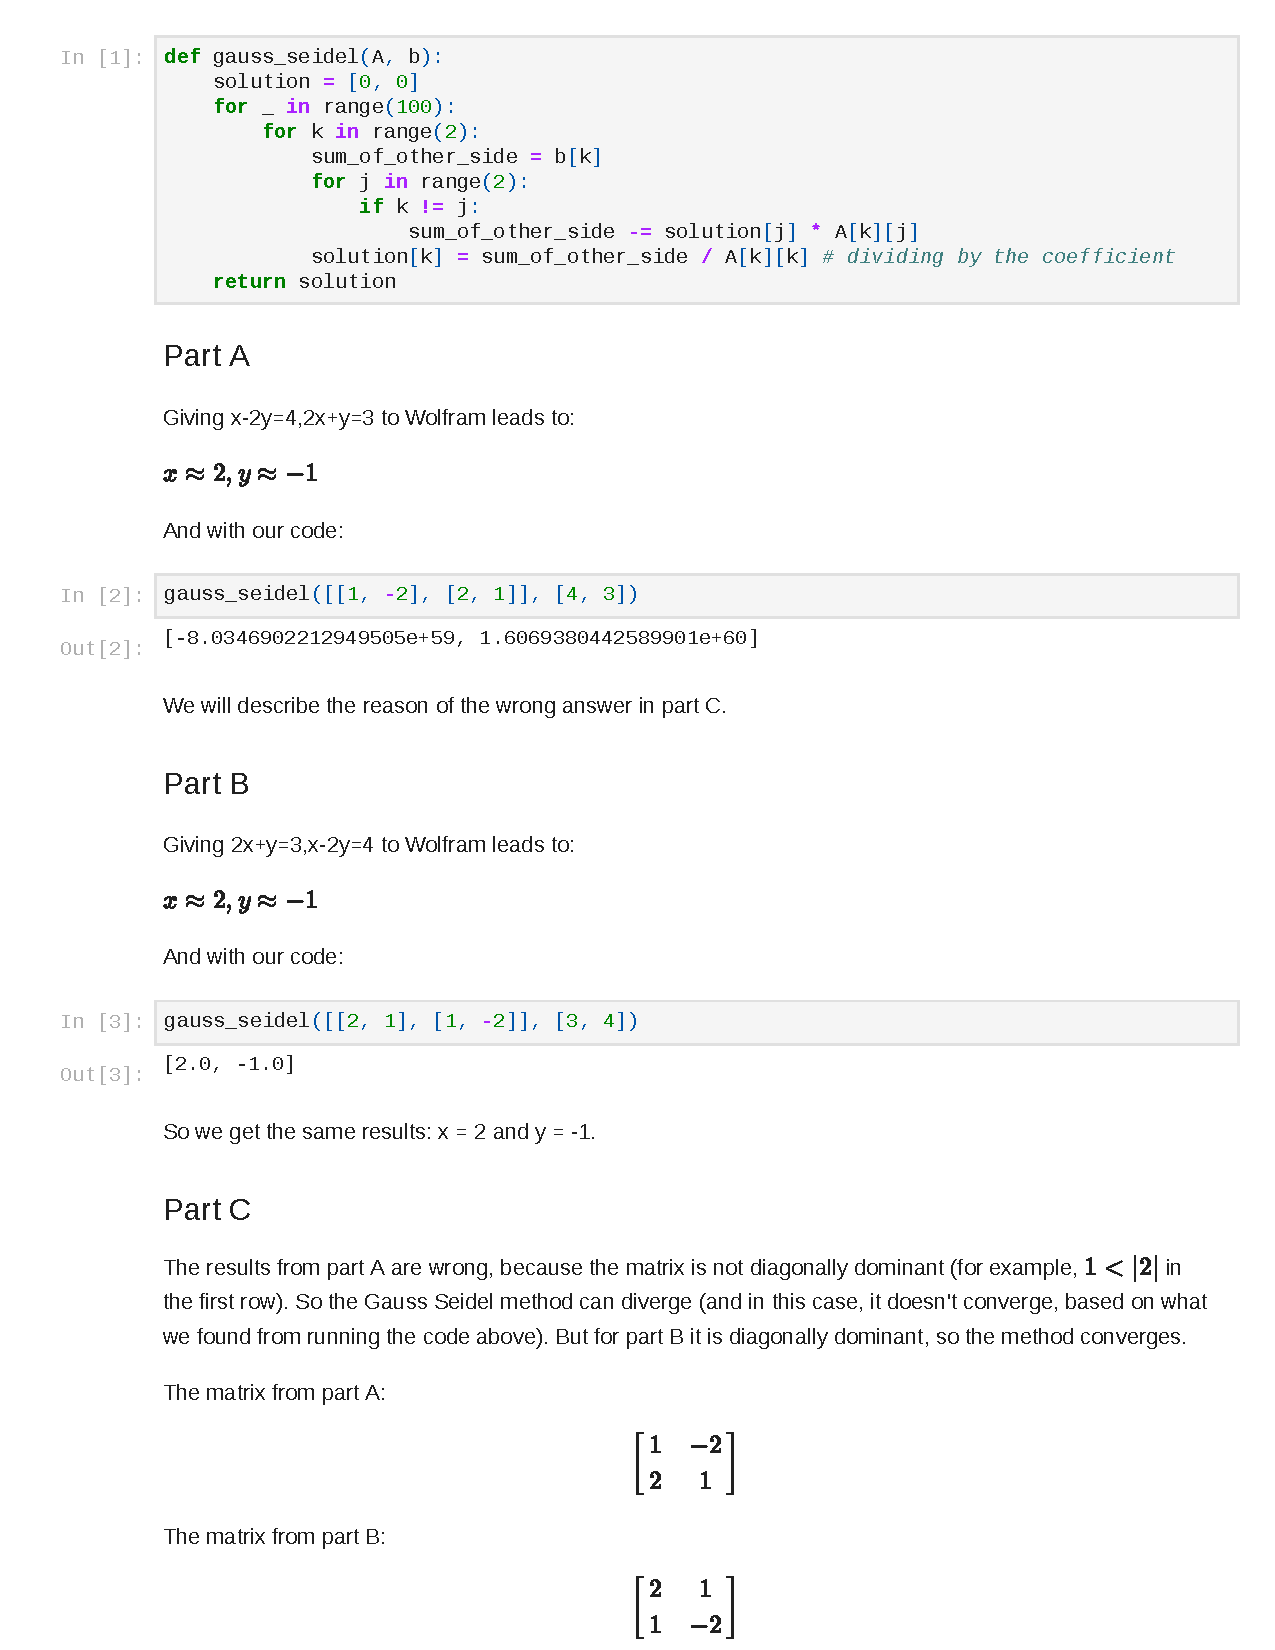
\includepdf[pages={1-},scale=1]{q5.pdf}
}